\documentclass[12pt,letterpaper]{article}

\usepackage{fancyhdr}
\pagestyle{fancy}
\fancyhf{}
\rhead{Vaja 7}
\lhead{ORS}
\setlength{\headheight}{16pt}

\usepackage[utf8]{inputenc}
\usepackage[slovene]{babel}
\usepackage[colorlinks = true, urlcolor = blue]{hyperref}

\usepackage{xcolor}
\usepackage{listings}
\usepackage{graphicx}
\graphicspath{{./images/}}
\definecolor{mGreen}{rgb}{0,0.6,0}
\definecolor{mGray}{rgb}{0.5,0.5,0.5}
\definecolor{mPurple}{rgb}{0.58,0,0.82}
\definecolor{backgroundColour}{rgb}{1,1,1}

\lstdefinestyle{CStyle}{
    backgroundcolor=\color{backgroundColour},
    commentstyle=\color{mGreen},
    keywordstyle=\color{magenta},
    numberstyle=\tiny\color{mGray},
    stringstyle=\color{mPurple},
    basicstyle=\footnotesize,
    breakatwhitespace=false,
    breaklines=true,
    captionpos=b,
    keepspaces=true,
    numbers=left,
    numbersep=5pt,
    showspaces=false,
    showstringspaces=false,
    showtabs=false,
    tabsize=2,
    language=C,
    frame=none
}

\begin{document}

\begin{center}
    \textbf{\Large Časovniki v STM32F4 (Cortex-M)}
\end{center}

Na tokratni vaji se bomo spoznali s časovniki, ki se uporabljajo za merjenje časa, izvajanje opravil v natančnih intervalih, programske zakasnitve, generiranje in prepoznavanje signalov s pulzno-dolžinsko modulacijo (PWM) ter še mnogo ostalih pogostih opravil povezanih s časom.

V splošnem imajo mikrokrmilniki STM32 tri različne tipe časovnikov: osnovne (angl. basic timers), splošno-namenske (angl. general-purpose timers) ter napredne časovnike (angl. advanced timers). Na tokratni vaji se bomo spoznali s principi delovanja splošno-namenskih časovnikov.

Mikrokrmilnik STM32F407, ki ga uporabljamo na vajah, ima na voljo 14 časovnikov, ki so označeni s predpono TIM ter številsko oznako. Časovnika TIM6 in TIM7 sta osnovnega tipa, časovnika TIM1 in TIM8 spadata med napredne časovnike, preostale (TIM2-TIM5, TIM9-TIM14) pa štejemo med splošno-namenske časovnike. Slednji se sicer med sabo še dodatno razlikujejo, vendar le v podrobnostih kot je velikost števcev, število kanalov in podobno. Koncept delovanja, ki je predstavljen v nadaljevanju, pa je enak za vse.


\section*{Osnovno delovanje časovnika}

Osnovni blok splošno-namenskih časovniko (angl. time-base unit) je prikazan na sliki \ref{timebase}. Glavna komponenta vsakega časovnika je števec, ki zna ob pozitivni urini fronti na vhodu prištevati ali odštevati stanje števca. Števec je v večini časovnikov 16-biten, razen pri TIM2 in TIM5, kjer je 32-biten. Frekvenca s katero šteje števec je določena z vhodno uro ter vrednostjo v delilniku ure (angl. prescaler). Slednji namreč deli frekvenco vhodne ure pred vhodom v števec ter števec tako upočasni.

\begin{figure}[ht!]
  \centering
  \caption{Osnovni blok časovnika (angl. time-base unit)}
  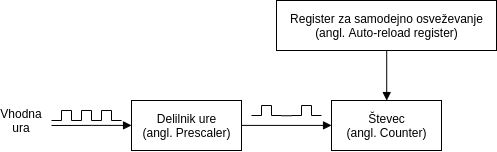
\includegraphics[width=280pt]{images/vaja7/timebase.png}
  \label{timebase}
\end{figure}

Vhodna ura časovnika je običajno ura vodila na katerem je priklopljen časovnik, lahko pa uporabimo tudi zunanjo ura, ki jo priklopimo na GPIO pin. V nadaljevanju predpostavljamo, da je vhodna ura časovnika ura vodila. Vsi časovniki so povezani na vodili APB1 in APB2. Na slednjem, na katerega so povezani časovniki TIM1, TIM8, TIM9 in TIM12, je najvišja možna frekvenca 168 MHz, kar je tudi glavna frekvenca mikrokrmilnika. Na vodilu APB1, na katerega so povezani preostali časovniki, pa je najvišja možna frekvenca polovica glavne frekvence mikrokrmilnika (84 MHz). 

V praznem projekt, kreiranem v STM32CubeIDE, sta obe omenjeni frekvenci nastavljeni na 16MHz. Spreminjate ju z dvoklikom na \texttt{.ioc} datoteko vašega projekta. V odprtem oknu nato izberete \texttt{Clock Configuration}. Ta vam odpre diagram prikazan na sliki \ref{timeconfig}. S spreminjamnjem vrednosti \texttt{APB1 Timer clocks} ter \texttt{APB1 Timer clocks} lahko spremenite frekvence vhodne ure časovnikov. Primeri v nadaljevanju predpostavljajo, da je vhodna frekvenca časovnika 16 MHz.

\begin{figure}[ht!]
  \centering
  \caption{Določanje frekvenc vhodnih ur časovnikov.}
  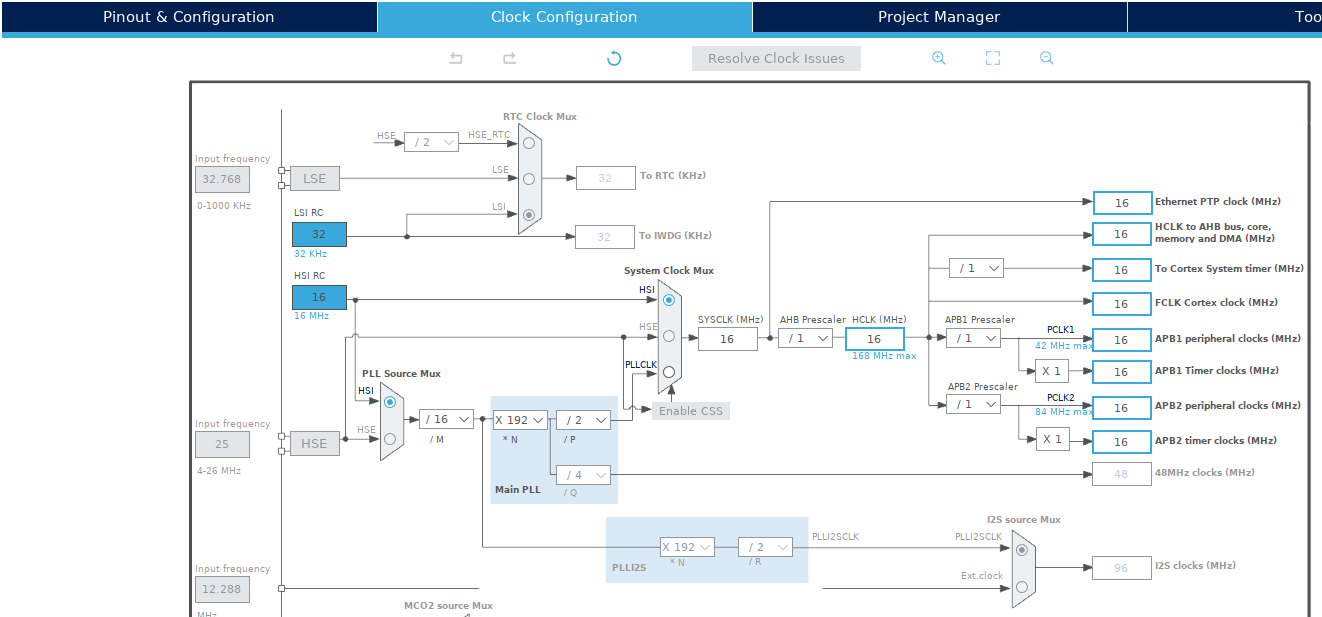
\includegraphics[width=380pt]{images/vaja7/clock_config.png}
  \label{timeconfig}
\end{figure}

Vhodna ura časovnika je, kot je vidno na sliki \ref{timebase} vhod v delilnik ure (angl. prescaler). Ta deli vhodno frekvenco z vrednostmi od 1 do 65536 (največje predstavljivo nepredznačeno 16-bitno število + 1). Če je delilnik ure nastavljen na vrednost 0, to pomeni, da se ura deli z 1, torej je frekvenca štetja enaka uri vodila. Če je delilnik ure nastavljen na vrednost 1, je frekvenca štetja polovica vhodne frekvence, in tako naprej do 65536, ki pomeni štetje s frekvenco $f = f_{vhod}/65537$. V splošnem je torej frekvenca enaka $f = f_{vhod}/(n + 1)$, kjer n predstavlja vrednost delilnika ure.

Števec lahko prišteva oziroma šteje navzgor (angl. upcounting mode), odšteva oziroma šteje navzdol (angl. downcounting mode) ali pa šteje navzgor in navzdol (angl. up/down counting ali center-aligned mode). V primeru štetja navzgor števec šteje od 0 do vključno vrednosti, ki je definirana v registru za samodejno osveževanje (angl. auto-reload register - ARR). Nato začne ponovno šteti od 0. V primeru štetja navzdol je začetno stanje števca enako ARR registru, ko doseže vrednost 0 pa začne ponovno šteti pri vrednosti definirani v registru ARR. V primeru štetja navzgor/navzdol števec šteje od 0 do ARR in nato nazaj od ARR do 0.

Sliki \ref{up_psc_0} in \ref{up_psc_1} prikazujeta dva diagrama štetja navzgor pri različnih vrednosti v delilniku ure (0 in 1). V obeh primerih je vrednost registra za samodejno osveževanje (ARR registra) 36. \texttt{CK\_INT} predstavlja vhodno uro časovnika, \texttt{CK\_CNT} predstavlja uro štetja, \texttt{Counter register} pa predstavlja stanje števca. Na diagramih lahko vidite tudi, da se ob ponovnem štetju z 0 pojavi tako imenovani update dogodek (angl. update event). Ob update dogodku se postavi zastavica (angl. flag), če želimo ob tem dogodku lahko prožimo tudi prekinitev. Prav tako se ob temu dogodku osveži nastavitev za ARR register. Če v program med izvajanjem želimo spremeniti vrednost ARR registra, se bo ta sprememba zgodila šele ob naslednjem update dogodku in ne takoj. Podobno velja za spremembe količnika za deljenje ure.

\begin{figure}[ht!]
  \centering
  \caption{Štetje navzgor brez deljenja ure in ARR = 36.}
  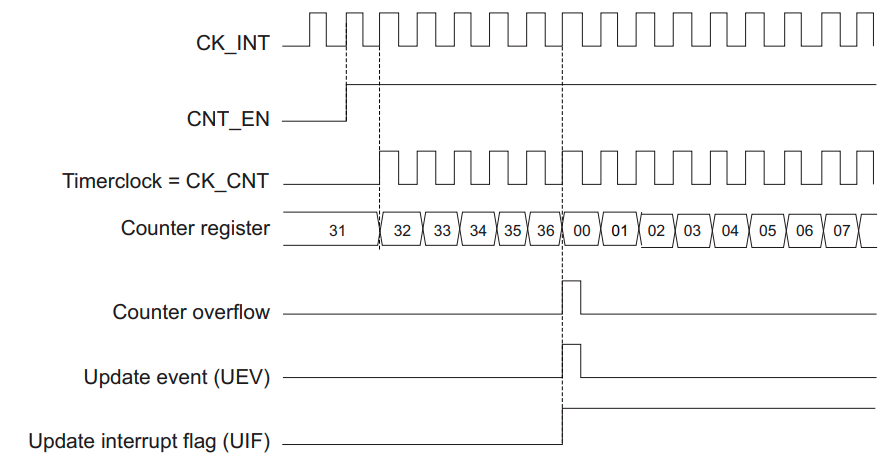
\includegraphics[width=360pt]{images/vaja7/prescaler0.png}
  \label{up_psc_0}
\end{figure}

\begin{figure}[ht!]
  \centering
  \caption{Štetje navzgor s polovično frekvenco in ARR = 36.}
  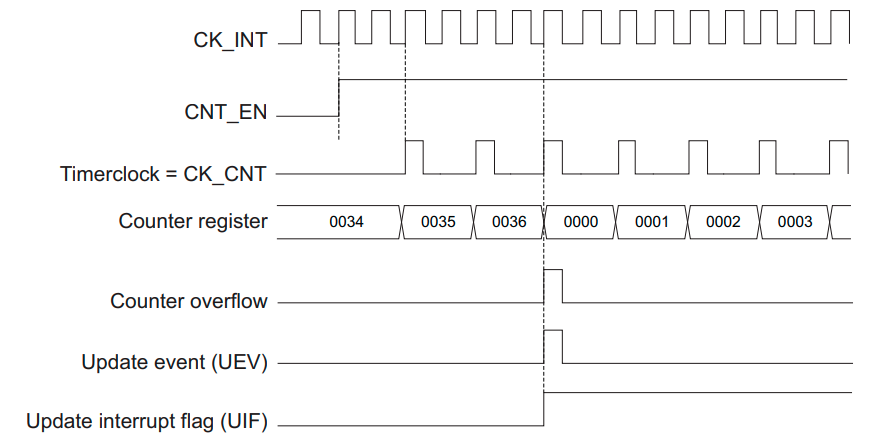
\includegraphics[width=350pt]{images/vaja7/prescaler1.png}
  \label{up_psc_1}
\end{figure}

Do sedaj opisane funkcionalnosti so vse kar ponujata osnovna časovnika TIM6 in TIM7. V nadaljevanju si poglejmo še dodatne funkcionalnosti, ki jih omogočajo splošno-namenski časovniki.


\section*{Kanali za zajem in primerjavo (angl. capture/compare channels)}

Vsi časovniki razen TIM6 in TIM7 imajo v časovniku na voljo kanale, ki omogočajo dodatne funkcionalnosti nad vhodnimi signali ter avtomatsko generiranje izhodnih signalov. Časovniki TIM1, TIM2, TIM3, TIM4, TIM5 in TIM8 imajo po 4 takšne ločene kanale, časovnika TIM9 in TIM12 imata oba po 2 kanala, preostali splošno-namenski časovniki pa po enega.

Na tokratni vaji se bomo osredotočili predvsem na izhodni del kanalov. Med vhodne funkcionalnosti, ki jih na tej vaji ne bomo spoznali, med drugim spadajo merjenje časa med dvema prehodoma na vhodni liniji, prepoznavanje frekvence ter dolžine pulza v signalu generiranem s pulzno-širinsko modulacijo (PWM).


\subsection*{Izhodni primerjalni način delovanja (angl. output compare mode)}

Osnovna funkcionalnosti časovnika, ki se ukvarja z izhodom, se imenuje output compare mode. Vsak kanal za zajem in primerjavo (angl. capture/compare channel) ima svoj register za primerjavo (angl. compare register). Ko števec časovnika doseže vrednost, ki je zapisana v tem registru, se kanal lahko odzove. Privzeti odziv je postavljanje zastavic CC1, CC2, CC3 in CC4 -- vsaka zastavica pripada enemu izmed štirih možnih kanalov. Ob postavljanju omenjenih zastavic se lahko proži tudi prekinitev ali neposredno nastavi stanje poljubnega GPIO pina. Vsak output compare kanal ima namreč fiksno določen GPIO pin, ki ga lahko ob odzivu kanala vsakič nastavi na logično vrednost 0, logično vrednost 1 ali pa negira trenutno logično vrednost na tem pinu (angl. toggle). V uporabniškem priročniku je jasno zapisano, kateri GPIO pin pripada kateremu izmed kanalov časovnikov. Na sliki \ref{oc_channel_gpio} lahko pri pinu PD12 vidite, da ima zapisano oznako \texttt{TIM4\_CH1}. To pomeni, da je ta pin povezan na prvi kanal TIM4. Preostali trije kanali istega časovnika so, kot lahko vidite, povezani na pine PD13, PD14 in PD15. Na naši razvojni plošči so ti pini, kot bi sedaj že morali vedeti, povezani na LED diode na razvojni plošči.

\begin{figure}[ht!]
  \centering
  \caption{GPIO pini kanalov časovnika.}
  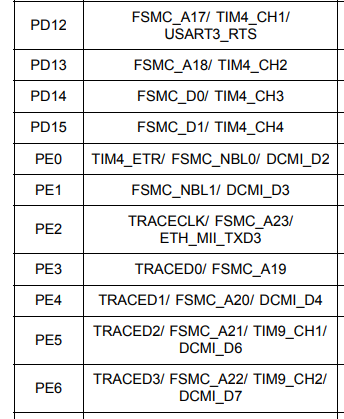
\includegraphics[width=170pt]{images/vaja7/oc_channel_gpio.png}
  \label{oc_channel_gpio}
\end{figure}

Odziv na kanal je lahko tudi proženje akcije druge naprave. Praktičen primer uporabe te funkcije je procesiranje zvočnih signalov, saj lahko s to funkcijo dosežemo vzorčenje vhodnega signala ob zelo natančnih intervalih.

\subsection*{Generiranje signala s pulzno-širinsko modulacijo}

Pulzno-širinska modulacija (angl. pulse-width modulation), ali na kratko PWM, je način kodiranja informacije z dolžino (širino) pulza. PWM signali imajo konstanto frekvenco in spreminjajočo dolžino pulza (glej sliko \ref{period_pulse}). Vsaka dolžina pulza ima lahko poseben pomen.

\begin{figure}[ht!]
  \centering
  \caption{Duty cycle PWM signala.}
  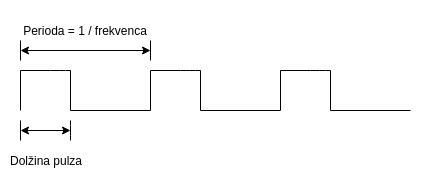
\includegraphics[width=250pt]{images/vaja7/perioda_pulz.png}
  \label{period_pulse}
\end{figure}

Frekvenca in dolžina pulza sta edini lastnosti, ki jih moramo določiti PWM signalom. Dolžino pulza pogosto opišemo s tako imenovanim ``duty cycleom'', ki je zapisan v odstotkih in pomeni kolikšen delež periode je signal aktiven. Če je signal celotno periodo neaktiven, je duty cycle 0\%. Petdesetodstotni duty cycle pa pomeni, da je signal aktiven polovico periode. Trije primeri so prikazani na sliki \ref{dutycycle}.

\begin{figure}[ht!]
  \centering
  \caption{Duty cycle PWM signala.}
  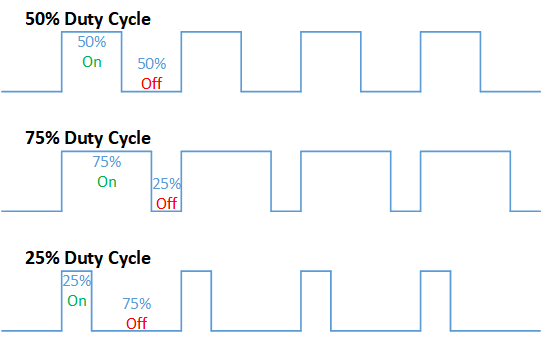
\includegraphics[width=250pt]{images/vaja7/dutycycle.png}
  \label{dutycycle}
\end{figure}

PWM signali se pogosto uporabljajo za krmiljenje servo motorjev. Servo motorji na primer zahtevajo PMW signal s frekvenco 50 Hz, kjer pulz dolžine 1 ms pomeni, da je motor obrnjen v eno smer, 2 ms pa pomeni, da je motor obrnjen v drugo smer.

Drug primer uporabe PWM signalov je zmanjšanje svetilnosti LED diod (angl. dimming). Pri stoodstotnem duty cyclu bo LED dioda svetila s polno svetilnostjo. Če pa duty cycle zmanjšamo, bo to za naše oko vidno kot da LED dioda sveti z zmanjšano svetilnostjo.


\section*{Knjižnica HAL in časovniki za STM32F4}

Pred inicializacijo časovnika moramo tako, kot vedno do sedaj, prižgati uro periferne naprave. Za časovnike to storimo z \texttt{\_\_HAL\_RCC\_TIMx\_CLK\_ENABLE()}. Pred tem v datoteki \texttt{Inc/stm32f4xx\_hal\_conf.h} odkomentirajte \texttt{HAL\_TIM\_MODULE\_ENABLED}.

\subsection*{Inicializacija osnovnega bloka}

Za inicializacijo osnovnega bloka časovnika določimo smer štetja, vrednost količnika delilnika ure (``prescalerja'') ter periodo štetja (vrednost v ARR registru). V strukturi v kateri določimo nastavitve, izberemo tudi časovnik. Če želimo uporabiti zgolj osnovni blok časovnika (time-base unit) inicializiramo časovnik s funkcijo \texttt{HAL\_TIM\_Base\_Init()}. Če želimo uporabiti časovnik za output compare, inicializiramo z \texttt{HAL\_TIM\_OC\_Init()}. \texttt{HAL\_TIM\_PWM\_Init()} uporabimo, če hočemo časovnik uporabiti za generiranje PWM signalov. Primer inicializacije je prikazan spodaj:

\begin{center}
\begin{lstlisting}[style=CStyle]
  __HAL_RCC_TIM3_CLK_ENABLE();

  TIM_HandleTypeDef timer;
  timer.Instance = TIM3;
  timer.Init.CounterMode = TIM_COUNTERMODE_UP;
  timer.Init.Period = 1000-1; // ARR 
  timer.Init.Prescaler = 16000-1;
  HAL_TIM_Base_Init(&timer);
  // ali HAL_TIM_OC_Init(&timer);
  // ali HAL_TIM_PWM_Init(&timer);
\end{lstlisting}
\end{center}

Prescaler je v tem primeru nastavljen na 16000-1. To pomeni, da je frekvenca štetja 1000 Hz. \texttt{Period} določa vrednost ARR registra. S temi nastavitvami se bo update dogodek pripetil vsako sekundo. Za nastavljene smeri štetja je možen nabor vrednosti:

\begin{itemize}
    \item \texttt{TIM\_COUNTERMODE\_UP}
    \item \texttt{TIM\_COUNTERMODE\_DOWN}
    \item \texttt{TIM\_COUNTERMODE\_CENTERALIGNED1}
    \item \texttt{TIM\_COUNTERMODE\_CENTERALIGNED2}
    \item \texttt{TIM\_COUNTERMODE\_CENTERALIGNED3}
\end{itemize}

\subsection*{Inicializacija output compare kanala}

Za osnovno delovanje output compare kanala zadostuje, da mu nastavimo vrednost compare registra. Primer takšne inicializacije je prikazan spodaj. \texttt{Pulse} je v tem primeru vrednost compare registra. Po spodnji inicializaciji in zagonu časovnika bi lahko brali stanje zastavice CC1 ali pa dodali, da se ob postavljanju zastavice CC1 proži prekinitev.

\begin{center}
\begin{lstlisting}[style=CStyle]
  TIM_OC_InitTypeDef OC_channel;
  OC_channel.Pulse = 500;
  HAL_TIM_OC_ConfigChannel(&timer, &OC_channel, TIM_CHANNEL_1);
\end{lstlisting}
\end{center}

Če želimo, da ob odzivu output compare kanal spremeni tudi stanje na pripadajočem izhodnem GPIO pinu moramo določiti še nastavitev \texttt{OCMode}, kjer lahko nastavimo, da kanal izhodni pin postavi na aktivno vrednost (\texttt{TIM\_OCMODE\_ACTIVE}), neaktivno logično vrednost (\texttt{TIM\_OCMODE\_INACTIVE}) ali pa stanje pina invertira (\texttt{TIM\_OCMODE\_TOGGLE}). Z nastavitvijo \texttt{OCPolarity} moramo še določiti ali je aktivna logična vrednost ničla \texttt{TIM\_OCPOLARITY\_LOW} ali enica \texttt{TIM\_OCPOLARITY\_HIGH}. Običajno je slednja nastavitev tista, ki smo je bolj vajeni. Primer obeh zgoraj opisanih opcij je prikazan spodaj. Poleg spodnje kode je potrebno ustrezno inicializirati tudi GPIO pin, ki pripada izbranem output compare kanalu časovnika. Več o nastavitvi GPIO pina je zapisano v nadaljevanju.

\begin{center}
\begin{lstlisting}[style=CStyle]
  TIM_OC_InitTypeDef OC_channel;
  OC_channel.OCMode = TIM_OCMODE_TOGGLE;
  OC_channel.OCPolarity = TIM_OCPOLARITY_HIGH;
  OC_channel.Pulse = 500;
  HAL_TIM_OC_ConfigChannel(&timer, &OC_channel, TIM_CHANNEL_1);
\end{lstlisting}
\end{center}


\subsection*{Inicializacija PWM izhoda}

Frekvenco PWM signala določimo z nastavitvijo količnika v delilniku vhodne ure ter nastavitvi ARR registra. To torej določimo ob inicializaciji osnovnega bloka. Frekvenca PWM signala je enaka frekvenci update dogodkov. Dolžino pulza pa določimo v compare kanalu z nastavitvijo compare registra. Če je njegova vrednost 0 gre za 0\% duty cycle. 100\% duty cycle dobimo, če compare register nastavimo na vrednost registra ARR. Kot pri inicializaciji output compare kanala tudi tu določimo katero logično vrednost ima signal, ko je aktiven. Primer inicializacije PWM izhoda je prikazan v primeru spodaj. Poleg spodnje inicializacije je zopet potrebno inicializirati tudi GPIO pin.

\begin{center}
\begin{lstlisting}[style=CStyle]
  TIM_OC_InitTypeDef PWM_channel;
  PWM_channel.OCMode = TIM_OCMODE_PWM1;
  PWM_channel.OCPolarity = TIM_OCPOLARITY_HIGH;
  PWM_channel.Pulse = 500;
  HAL_TIM_PWM_ConfigChannel(&timer, &PWM_channel, TIM_CHANNEL_1);
\end{lstlisting}
\end{center}

Način delovanja \texttt{TIM\_OCMODE\_PWM1} je običajen PWM signal, kot je prikazan na sliki \ref{period_pulse}, kjer je prvi del periode pulz, temu pa sledi neaktiven del periode. Pri \texttt{TIM\_OCMODE\_PWM2} je pulz na koncu periode.

\subsection*{Inicializacija GPIO}

GPIO pine, s katerimi neposredno upravlja časovnik, moramo inicializirati v načinu alternativne funkcije (AF), s tem pine ne uporabljamo kot klasičen GPIO vhod ali izhod, ampak jih predamo v uporabo časovniku. Za določitev alternativnih funkcij si pomagajte z inicializacijo GPIO pinov pri peti vaji. Slika \ref{SPI_AF} naj vam bo v pomoč pri izbiri alternativne funkcije.

\begin{figure}[ht!]
  \centering
  \caption{Mapiranje alternativnih funkcij.}
  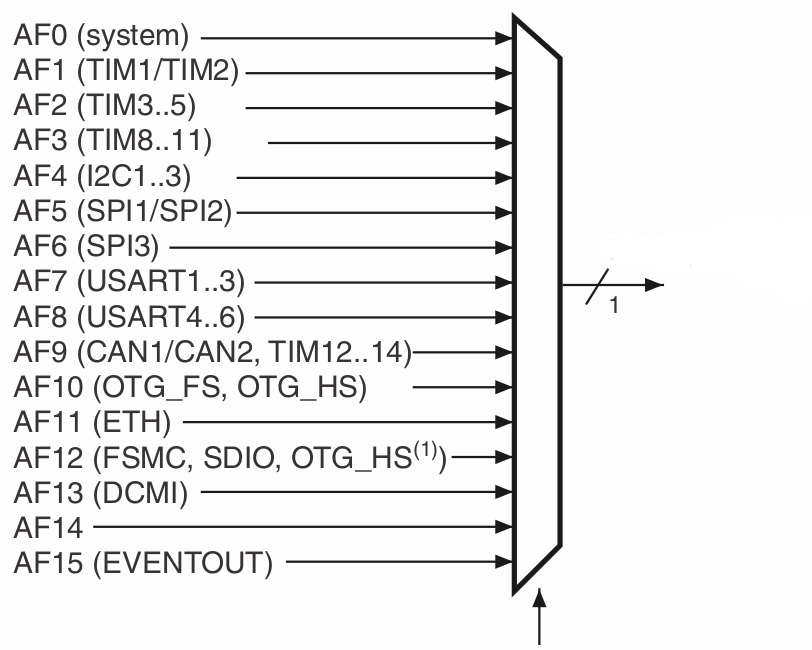
\includegraphics{images/vaja5/SPI_AF.png}
  \label{SPI_AF}
\end{figure}

\subsection*{Upravljanje časovnika}

Po inicializaciji je potrebno časovnik še zagnati. Spodaj so prikazani primeri zagona časovnika, pri uporabi osnovnega bloka, output compare kanala ter generiranja PWM signala.

\begin{center}
\begin{lstlisting}[style=CStyle]
  HAL_TIM_Base_Start(&timer);
  HAL_TIM_OC_Start(&timer, TIM_CHANNEL_1);
  HAL_TIM_PWM_Start(&timer, TIM_CHANNEL_2);
\end{lstlisting}
\end{center}

Med delovanjem časovnika lahko spreminjamo določene nastavitve. Najpogosteje spreminjamo vrednost compare registra ali količnika delilnika ure. Seznam funkcij in primeri uporabe so podani spodaj.

\begin{center}
\begin{lstlisting}[style=CStyle]
  __HAL_TIM_SET_PRESCALER(&timer, 1000);
  __HAL_TIM_SET_COUNTER(&timer, 1000);
  __HAL_TIM_SET_AUTORELOAD(&timer, 1000);
  __HAL_TIM_SET_COMPARE(&timer, TIM_CHANNEL_1, 1000);
\end{lstlisting}
\end{center}

\subsection*{Zastavice časovnikov}

Časovniki imajo množico zastavic, s katerimi lahko spremljate njihovo stanje. Za nas je zanimivih spodnjih 5, ki označujejo update dogodek ter odzive vseh štirih možnih output compare kanalov.

\begin{center}
\begin{lstlisting}[style=CStyle]
  TIM_FLAG_UPDATE
  TIM_FLAG_CC1
  TIM_FLAG_CC2
  TIM_FLAG_CC3
  TIM_FLAG_CC4
\end{lstlisting}
\end{center}

Zastavice lahko preverjamo s funckijo \texttt{\_\_HAL\_TIM\_GET\_FLAG()}, ki ji podamo kazalec na strukturo časovnika ter oznako zastavice. Enake argumente ima tudi funckija za brisanje zastavic \texttt{\_\_HAL\_TIM\_CLEAR\_FLAG()}.

\subsection*{Prekinitve časovnikov}

Časovniku lahko omogočimo, da ob katerikoli izmed zgornjih zastavic proži prekinitev. Prekinitev omogočimo z ukazom \texttt{\_\_HAL\_TIM\_ENABLE\_IT()}, ki mu podamo kazalec na strukturo časovnika ter oznako prekinitve. Oznake prekinitev so podobne imenom zastavic:

\begin{center}
\begin{lstlisting}[style=CStyle]
  TIM_IT_UPDATE
  TIM_IT_CC1
  TIM_IT_CC2
  TIM_IT_CC3
  TIM_IT_CC4
\end{lstlisting}
\end{center}

Poleg vklopa prekinitve v časovniku, moramo prekinitve omogočiti tudi v prekinitvenem krmilniku, enako kot pri prejšnji vaj za zunanje prekinitve (EXTI). Primer vklopa prekinitev za časovnik TIM3 je podan spodaj.

\begin{center}
\begin{lstlisting}[style=CStyle]
  HAL_NVIC_SetPriority(TIM3_IRQn, 0, 1);
  HAL_NVIC_EnableIRQ(TIM3_IRQn); 
\end{lstlisting}
\end{center}

Spodnja tabela vsebuje seznam vse prekinitvenih oznak ter imen prekinitveno servisnih programov za časovnike. Kot vidite ima vsak od naprednih časovnikov več prekinitvenih oznak, splošno namenski ter osnovna časovnika pa zgolj po eno. Časovniki TIM9-TIM14 si prekinitvene oznake delijo s TIM1 in TIM8. V prekinitveno servisnem programu preverjamo in brišemo prekinitvene zahteve s funkcijami za delo z zastavicami (kot pri prejšnji vaji).
\begin{center}
\begin{table}[ht!]
\small
\begin{tabular}{|c|c|c|}
\hline
Časovnik & Prekinitvene oznake                                                                                                                      & Imena PSP-jev                                                                                                                                                      \\ \hline
TIM1     & \begin{tabular}[c]{@{}c@{}}TIM1\_BRK\_TIM9\_IRQn,\\ TIM1\_UP\_TIM10\_IRQn,\\ TIM1\_TRG\_COM\_TIM11\_IRQn,\\ TIM1\_CC\_IRQn\end{tabular}  & \begin{tabular}[c]{@{}c@{}}TIM1\_BRK\_TIM9\_IRQHandler,\\ TIM1\_UP\_TIM10\_IRQHandler,\\ TIM1\_TRG\_COM\_TIM11\_IRQHandler,\\ TIM1\_CC\_IRQHandler\end{tabular} \\ \hline
TIM2     & TIM2\_IRQn                                                                                                                               & TIM2\_IRQHandler                                                                                                                                                   \\ \hline
TIM3     & TIM3\_IRQn                                                                                                                               & TIM3\_IRQHandler                                                                                                                                                   \\ \hline
TIM4     & TIM4\_IRQn                                                                                                                               & TIM4\_IRQHandler                                                                                                                                                   \\ \hline
TIM5     & TIM5\_IRQn                                                                                                                               & TIM5\_IRQHandler                                                                                                                                                   \\ \hline
TIM6     & TIM6\_DAC\_IRQn                                                                                                                          & TIM6\_DAC\_IRQHandler                                                                                                                                              \\ \hline
TIM7     & TIM7\_IRQn                                                                                                                               & TIM7\_IRQHandler                                                                                                                                                   \\ \hline
TIM8     & \begin{tabular}[c]{@{}c@{}}TIM8\_BRK\_TIM12\_IRQn,\\ TIM8\_UP\_TIM13\_IRQn,\\ TIM8\_TRG\_COM\_TIM14\_IRQn,\\ TIM8\_CC\_IRQn\end{tabular} & \begin{tabular}[c]{@{}c@{}}TIM8\_BRK\_TIM12\_IRQHandler,\\ TIM8\_UP\_TIM13\_IRQHandler,\\ TIM8\_TRG\_COM\_TIM14\_IRQHandler,\\ TIM8\_CC\_IRQHandler\end{tabular}   \\ \hline
TIM9     & TIM1\_BRK\_TIM9\_IRQn                                                                                                                    & TIM8\_UP\_TIM13\_IRQHandler                                                                                                                                        \\ \hline
TIM10    & TIM1\_UP\_TIM10\_IRQn                                                                                                                    & TIM8\_TRG\_COM\_TIM14\_IRQHandler                                                                                                                                  \\ \hline
TIM11    & TIM1\_TRG\_COM\_TIM11\_IRQn                                                                                                              & TIM8\_CC\_IRQHandler                                                                                                                                               \\ \hline
TIM12    & TIM8\_BRK\_TIM12\_IRQn                                                                                                                   & TIM8\_BRK\_TIM12\_IRQHandler                                                                                                                                       \\ \hline
TIM13    & TIM8\_UP\_TIM13\_IRQn                                                                                                                    & TIM8\_UP\_TIM13\_IRQHandler                                                                                                                                        \\ \hline
TIM14    & TIM8\_TRG\_COM\_TIM14\_IRQn                                                                                                              & TIM8\_TRG\_COM\_TIM14\_IRQHandler                                                                                                                                  \\ \hline
\end{tabular}
\end{table}
\end{center}
\newpage
\section*{Naloga}

Časovnik TIM4 nastavite tako, da bo generiral PWM signale za vse štiri LED diode. Ob zagonu naj 2 LED diodi po vaši izbiri (LED1 in LED2) svetita s polno svetilnostjo, preostali 2 (LED3 in LED4) pa naj bosta ugasnjeni (0\% duty cycle).

Nato uporabite enega izmed preostalih časovnikov za proženje prekinitev. Nastavite ga tako, da se bo prekinitev sprožila vsakih 50 ms. Ob prekinitvi spreminjajte duty cycle za LED1 in LED2 tako da najprej zmanjšujete svetilnost dokler nista popolnoma ugasnjeni, nato pa jima svetilnost povečujte nazaj do polne svetilnost. Pri LED 3 in LED 4 duty cycle spreminjajte v obratni smeri, torej najprej ga povečujete, pri polni svetilnosti pa ga začnete zmanjševati. Takšno ``neskončno'' osciliranje LED diod je tudi končna rešitev naloge.

\end{document}
